\documentclass[conference]{IEEEtran}
\IEEEoverridecommandlockouts
% The preceding line is only needed to identify funding in the first footnote. If that is unneeded, please comment it out.
\usepackage{cite}
\usepackage{amsmath,amssymb,amsfonts}
\usepackage{graphicx}
\usepackage{multicol}
\usepackage{caption}
\usepackage{subcaption}
\usepackage{caption}
\usepackage{textcomp}
\usepackage{xcolor}
\usepackage{url}
\usepackage[czech]{babel}
\usepackage{siunitx}

\graphicspath{{./images}}
\usepackage{caption}
\captionsetup[subfigure]{justification=centering} %configure subfigures to use centered captions
\captionsetup[figure*]{justification=centering} %configure subfigures to use centered captions

\def\BibTeX{{\rm B\kern-.05em{\sc i\kern-.025em b}\kern-.08em
    T\kern-.1667em\lower.7ex\hbox{E}\kern-.125emX}}
\begin{document}


\title{Automatické řízení - semestrální úloha}

\author{\IEEEauthorblockN{Vojtěch Michal}
michavo3@fel.cvut.cz}

\maketitle

\begin{abstract}
Report z modelování, analýzy a návrhu řízení pro dvoukolový segway postavený s vývojovou sadou LEGO Mindstorms.
Cílem práce je stabilizace segwaye v nestabilním svislém ekvilibriu a pohyb po rovné čáře.
\end{abstract}

\begin{IEEEkeywords}
    identifikace, linearizace, stabilizace, řízení, LEGO segway
\end{IEEEkeywords}

\section{Úvod}
\label{sec:uvod}
Segway je dvoukolové vozítko. Protože je těžiště umístěno nad osou otáčení, je nezbytné jej ve svislém nestabilním
ekvilibriu aktivně udržovat pomocí řízení. Cílem úlohy je analyzovat model segwaye a navrhnout pro něj řízení. 

\begin{figure}[htbp]
    \centerline{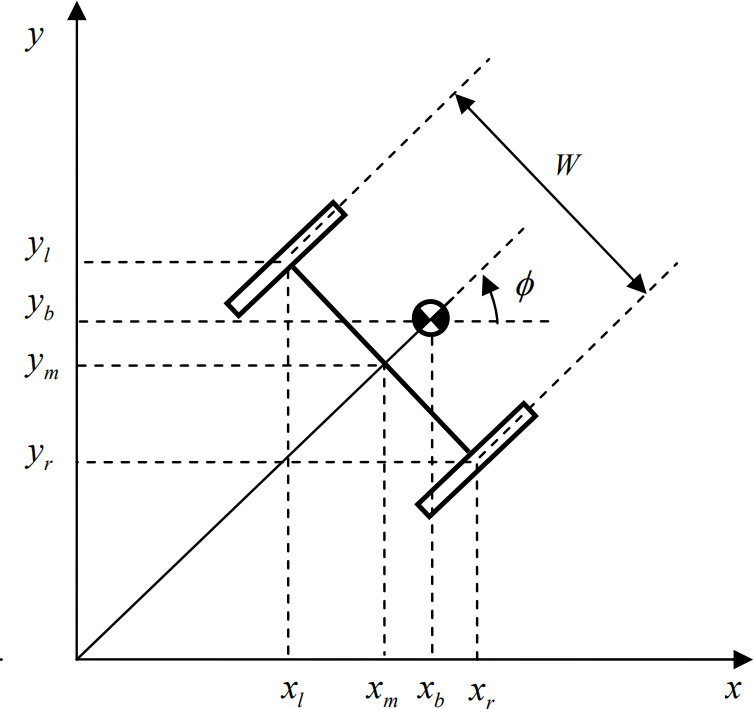
\includegraphics[width=0.9\linewidth]{segway_shora.png}}
    \caption{Nákres segwaye shora, zapůjčeno z \cite{model_based_design}}
    \label{fig:segway_shora}        
\end{figure}

\begin{figure}[htbp]
    \centerline{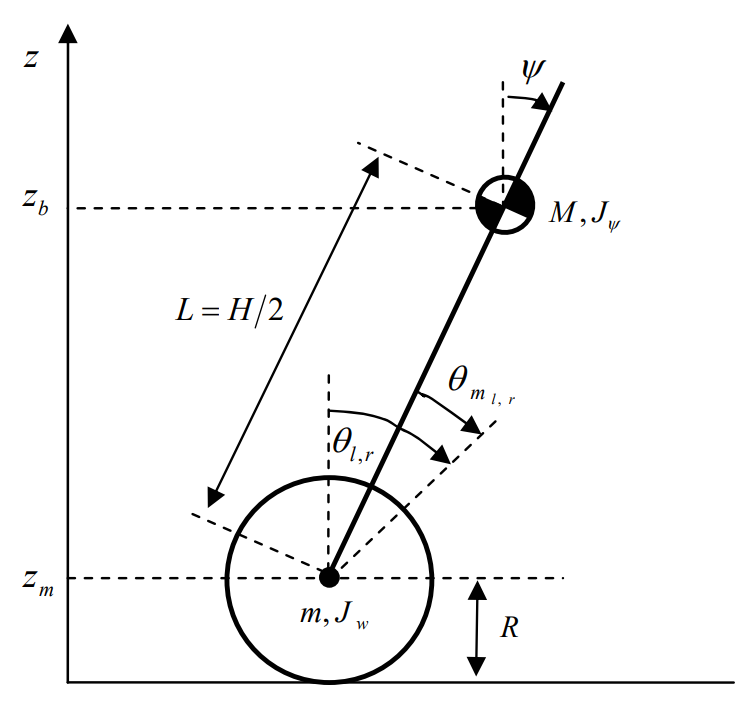
\includegraphics[width=0.9\linewidth]{segway_bok.png}}
    \caption{Nákres segwaye z boku, zapůjčeno z \cite{model_based_design}}
    \label{fig:segway_bok}        
\end{figure}

\section{Matematický model}
Na obrázcích \ref{fig:segway_bok} a \ref{fig:segway_shora} je zaveden souřadný systém a vyznačen význam dalších veličin
nezbytných pro matematický popis segwaye. Odvození matematického modelu je založeno na \cite{model_based_design}.
Uvažujeme tři zobecněné souřadnice
\begin{equation*}
    \begin{aligned}
        \frac{\theta_l + \theta_r}{2} = \theta~ [\si{rad}] &\cdots \text{Průměrný úhel levého a pravého kola,} \\
        \psi ~[\si{rad}] &\cdots \text{Náklon segwaye (otáčení v ose koleček),} \\
        \varPhi~[\si{rad}] &\cdots \text{Azimut segwaye (svislá osa otáčení).}
    \end{aligned}
\end{equation*}



Tabulka \ref{tab:konstanty} shrnuje všechny konstantní parametry použité při modelování systému včetně jejich hodnot.
Některé konkrétní hodnoty jsou převzaty z \cite{model_based_design}, část hodnot ovšem bylo možno experimentálně ověřit.
Hmotnost koleček $m$, hmotnost segwaye $M$, šířka vozítka $W$, tloušťka $D$ i výška $H$ se odlišují od hodnot
představených v \cite{model_based_design}. Rovněž byl přeměřen poloměr koleček $R$.
Dále jsou v tabulce \ref{tab:konstanty} zaneseny změřené hodnoty maximálního napětí baterie $U_\text{max}$ po plném nabití,
vnitřního odpor baterie $R_\text{in}$ a velikosti napájecího proudu při plném výkonu motorů $I_\text{max}$.

\begin{table}[htbp]
    \centering
    \begin{tabular}[t]{|c|c|c|}
        \hline
        symbol & valikost & veličina \\\hline
        g  & 9.81 \si{m/s} & Gravitační zrychlení \\\hline
        $ m $ & 0.012 \si{kg} & Hmotnost kolečka \\\hline
        $ R $ & 0.04 \si{m }& Poloměr kolečka \\\hline
        $ J_w $ & $\frac{mR^2}{2}$ \si{kg . m^2} & Moment setrvačnosti kolečka \\\hline
        $ M $ & 0.58   \si{kg} & Hmotnost segwaye \\\hline
        $ W $ & 0.17  \si{ m} & Šířka segwaye (délka ve směru osy rotace kol) \\\hline
        $ D $ & 0.055  \si{ m} & Tloušťka segwaye (délka ve směru pohybu) \\\hline
        $ H $ & 0.16 \si{m }& Výška  segwaye \\\hline
        $ L $ & $\frac{H}{2}$ \si{m} & Vzdálenost těžiště segwaye od osy kol \\\hline
        $ J_\psi $ & $\frac{ML^2}{3}$ \si{kg . m^2} & Moment setrvačnosti náklonu segwaye\\\hline
        $ J_\varPhi $ & $\frac{M(W^2 + D^2)}{12}$ \si{kg . m^2} & Moment setrvačnosti rotace segwaye \\\hline
        $ J_m $ & $10^{-5}$ \si{kg . m^2} & Moment setrvačnosti motoru \\\hline
        $ R_m $ & 6.69 $\Omega$ & Odpor motoru \\\hline
        $ K_b $ & 0.468 \si{V.s/rad} & EMF kontanta motoru \\\hline
        $ K_t $ & 0.317 \si{Nm/A} & Konstanta kroutivého momentu motoru \\\hline
        $ n $ & 1 [-] & Převodní poměr převodovky \\\hline
        $ f_m $ & 0.0022 [-] & Koeficient tření mezi motorem a segwayem \\\hline
        $ f_w $ & 0 [-] & Koeficient tření mezi kolem a podložkou \\\hline
        $ U_\text{max} $ & 8.3 \si{V} & Maximální mapětí napájecí baterie \\\hline
        $ R_\text{in} $ & 0.65 \si{\ohm} & Vnitřní odpor baterie \\\hline
        $ I_\text{max} $ & 300 \si{\milli\ampere} & Špičkový napájecí proud \\\hline
        
    \end{tabular}
    \caption{Konstantní parametry modelu segwaye}
    \label{tab:konstanty}
\end{table}

\pagebreak
\subsection{Nelineární rovnice}
Pomocí analýzy geometrie úlohy lze určit Lagrangián a jeho derivováním podle zobecnělých souřadnic 
následně pro soustavu sestavit obecné pohybové rovnice \eqref{eq:pohyb1}, \eqref{eq:pohyb2} a \eqref{eq:pohyb3}.

\begin{equation}
    \begin{aligned}
        &\left[(2m + M) R^2 + 2 J_w + 2n^2 J_m\right] \ddot{\theta} + \\
        &+ (MLR \text{cos} \psi - 2n^2 J_m) \ddot{\psi} - MLR\dot{\psi}^2 \text{sin} \psi = F_\theta,
    \end{aligned}
    \label{eq:pohyb1}
\end{equation}
\begin{equation}
    \begin{aligned}
        & (MLR \text{cos} \psi - 2n^2 J_m) \ddot{\theta} + (ML^2 + J_\psi + 2n^2 J_m) \ddot{\psi} - \\
        & - MgL\text{sin}\psi - ML^2\dot{\varPhi}^2 \text{sin} \psi \text{cos} \psi = F_\psi,
    \end{aligned}
    \label{eq:pohyb2}
\end{equation}
\begin{equation}
    \begin{aligned}
        &\left[ \frac{1}{2} mW^2  + J_\varPhi + \frac{W^2}{2R^2}\left( J_w + n^2 J_m \right) + ML^2 \text{sin}^2 \psi \right] \ddot{\varPhi} + \\
        &+ 2ML^2 \dot{\psi} \dot{\varPhi} \text{sin}\psi \text{cos} \psi = F_\varPhi.
    \end{aligned}
    \label{eq:pohyb3}
\end{equation}

Zobecněné síly na pravé straně rovnic lze vyjádřit jako
\begin{equation}
    F_\theta = \alpha(v_l + v_r) - 2(\beta + f_w) \dot{\theta} + 2\beta\dot{\psi},
    \label{eq:motor1}
\end{equation}
\begin{equation}
    F_\psi = -\alpha(v_l + v_r) + 2\beta \dot{\theta} - 2\beta \dot{\psi},
    \label{eq:motor2}
\end{equation}
\begin{equation}
    F_\varPhi = \frac{W}{2R} \alpha (v_l - v_r) - \frac{W^2}{2R^2}(\beta + f_w) \dot{\varPhi},
    \label{eq:motor3}
\end{equation}
kde symboly $\alpha$ a $\beta$ jsou substitucemi za výrazy
\begin{equation}
    \begin{split}
        \alpha &= \frac{n \cdot K_t} {R_m},  \\
        \beta &= \frac{n \cdot K_t \cdot K_b} {R_m} + f_m .
    \end{split}
    \label{eq:motor_substituce}
\end{equation}

\subsection{Základní úpravy modelu}
S ohledem na charakter úlohy popsané v sekci \ref{sec:uvod} si lze dovolit dvě základní zjednodušení. Protože segway
má pouze balancovat nebo jezdit po rovné čáře, bude jeho azimut $\varPhi$ vždy konstantní. 
Bez újmy na obecnosti lze postavit dokonce $\varPhi = 0$ (odtud i $\dot{\varPhi} = \ddot{\varPhi} = 0$),
čímž se z modelu úplně eliminuje rovnice \eqref{eq:pohyb3}
a rovnice \eqref{eq:pohyb2} se zjednoduší vynulováním jednoho sčítance. Zároveň již není potřeba pracovat se silou $F_\varPhi$
a rovnice \eqref{eq:motor3} tak též může být odstraněna.

Další zjednodušní plyne z rozhodnutí řídit levý i pravý motor stejným napětím $v_l = v_r = v$.
Toto zjednodušení má vliv na rovnice \eqref{eq:motor1} a \eqref{eq:motor2}.

Součástí druhé úlohy je rovněž regulace vzdálenosti od překážky $d(t)$.
Protože vzdálenost svazuje s proměnnou $\theta(t)$ vzájemně jednoznačný vztah
\begin{equation}
    \Delta d(t) = R \Delta\theta(t),
    \label{eq:vzdalenost}
\end{equation}
není nezbytné přidávat vzdálenost $d$ jako další stav robota, neboť se jedná o lineární funkci již existujícícho stavu $\theta$.

Nová sada rovnic popisujících systém má tvar
\begin{equation}
    \begin{aligned}
        &\left[(2m + M) R^2 + 2 J_w + 2n^2 J_m\right] \ddot{\theta} + \\
        &+ (MLR \text{cos} \psi - 2n^2 J_m) \ddot{\psi} - MLR\dot{\psi}^2 \text{sin} \psi = F_\theta,
    \end{aligned}
    \label{eq:pohyb1_easy}
\end{equation}
\begin{equation}
    \begin{aligned}
        & (MLR \text{cos} \psi - 2n^2 J_m) \ddot{\theta} + \\
        & + (ML^2 + J_\psi + 2n^2 J_m) \ddot{\psi} - MgL\text{sin}\psi = F_\psi,
    \end{aligned}
    \label{eq:pohyb2_easy}
\end{equation}

\begin{equation}
    F_\theta = 2v \alpha - 2(\beta + f_w) \dot{\theta} + 2\beta\dot{\psi},
    \label{eq:motor1_easy}
\end{equation}
\begin{equation}
    F_\psi = - 2v \alpha + 2\beta \dot{\theta} - 2\beta \dot{\psi},
    \label{eq:motor2_easy}
\end{equation}

\subsection{Linearizace}
\label{sec:linearizace}

Základním cílem úlohy je stabilizace robota ve svislé poloze, což je zvolený pracovní bod.
Platí pro něj $\psi_p = 0$. Na konkrétní úhel natočení koleček $\theta_p$ není třeba klást žádný požadavek,
protože úloha je translačně invariantní a fyzika segwaye nezávisí na tom, jakou vzdálenost již urazil.
Bez újmy na obecnosti lze zvolit $\theta_p = 0$, protože se tento stav stejně v žádné rovnici přímo nevyskytuje.

V okolí pracovního bodu lze provést aproximaci $\text{cos}(\psi) \approx 1$, $\text{sin}(\psi) \approx \psi$. Rovněž výraz $\dot{\psi}^2$ se bude limitně blížit nule,
protože pro stabilní systém není žádoucí velká úhlová rychlost. Rovnice \eqref{eq:pohyb1_easy} a \eqref{eq:pohyb2_easy} se zjednoduší na
\begin{equation}
    \left[(2m + M) R^2 + 2 J_w + 2n^2 J_m\right] \ddot{\theta} + (MLR - 2n^2 J_m) \ddot{\psi} = F_\theta,
    \label{eq:pohyb1_lin}
\end{equation}
\begin{equation}
    (MLR - 2n^2 J_m) \ddot{\theta} + (ML^2 + J_\psi + 2n^2 J_m) \ddot{\psi} - MgL \psi = F_\psi.
    \label{eq:pohyb2_lin}
\end{equation}

Pro zjednodušení rovnic \eqref{eq:pohyb1_lin}, \eqref{eq:pohyb2_lin}, \eqref{eq:motor1_easy} a \eqref{eq:motor2_easy}
je možné sdružit konstantní koeficienty do nových 
\begin{equation}
    \begin{split}
        l_1 &= (2m + M) R^2 + 2 J_w + 2n^2 J_m, \\
        l_2 &= MLR - 2n^2 J_m, \\
        l_3 &= ML^2 + J_\psi + 2n^2 J_m, \\
        l_4 &= MgL, \\
        c_1 &= 2(\beta + f_w).
    \end{split}
\end{equation}
S tímto označením mají linearizované rovnice tvar
\begin{equation}
    l_1 \ddot{\theta} + l_2 \ddot{\psi} = 2v \alpha - c_1 \dot{\theta} + 2\beta\dot{\psi},
    \label{eq:pohyb1_lin_simple}
\end{equation}
\begin{equation}
    l_2 \ddot{\theta} + l_3 \ddot{\psi} - l_4 \psi = - 2v \alpha + 2\beta \dot{\theta} - 2\beta \dot{\psi}.
    \label{eq:pohyb2_lin_simple}
\end{equation}

Pro získání stavových rovnic je nezbytné osamostatnit z \eqref{eq:pohyb1_lin_simple} a \eqref{eq:pohyb2_lin_simple}
druhé derivace veličin $\theta$ a $\psi$. Analytické řešení vede na vztahy
\begin{equation}
    \begin{split}
        \ddot{\theta} & = \frac{2\beta (l_2 + l_3) \dot{\psi}  - (2 \beta l_2 + c_1 l_3) \dot{\theta} - l_2 l_4 \psi + 2 \alpha (l_2 + l_3) v}{l_1 l_3 - l_2^2}, \\
        \ddot{\psi} &= \frac{- 2 \beta (l_1 + l_2) \dot{\psi} + (2 \beta l_1 + c_1 l_2)\dot{\theta}  + l_1 l_4 \psi - 2 \alpha (l_1 + l_2) v}{l_1 l_3 - l_2^2},
        \label{eq:druhe_derivace}
    \end{split}
\end{equation}
které lze dále zjednodušit sdružením kostantních parametrů. Zavedením označení
\begin{equation*}
    a_1 = \frac{2\beta (l_2 + l_3)}{l_1 l_3 - l_2^2}, \\
\end{equation*}
\begin{equation*}
    a_2 = -\frac{2 \beta l_2 + c_1 l_3}{l_1 l_3 - l_2^2}, \\
\end{equation*}
\begin{equation*}
    a_3 = -\frac{l_2 l_4}{l_1 l_3 - l_2^2}, \\
\end{equation*}
\begin{equation*}
    a_4 = \frac{2 \alpha (l_2 + l_3)}{l_1 l_3 - l_2^2}, \\
\end{equation*}
\begin{equation*}
    a_5 = -\frac{2 \beta (l_1 + l_2)}{l_1 l_3 - l_2^2}, \\
\end{equation*}
\begin{equation*}
    a_6 = \frac{2 \beta l_1 + c_1 l_2}{l_1 l_3 - l_2^2}, \\
\end{equation*}
\begin{equation*}
    a_7 = \frac{ l_1 l_4 }{l_1 l_3 - l_2^2}, \\
\end{equation*}
\begin{equation*}
    a_8 = -\frac{2 \alpha (l_1 + l_2)}{l_1 l_3 - l_2^2}, \\
\end{equation*}
se rovnice \eqref{eq:druhe_derivace} zjednoduší na
\begin{equation}
    \begin{split}
        \ddot{\theta} & = a_1 \dot{\psi} + a_2  \dot{\theta} + a_3  \psi + a_4  v, \\
        \ddot{\psi} &= a_5  \dot{\psi} + a_6  \dot {\theta} + a_7  \psi + a_8  v.
        \label{eq:druhe_derivace_easy}
    \end{split}
\end{equation}

Přeznačme fyzikální veličiny v rovnici \eqref{eq:druhe_derivace_easy} podle konvence v oboru automatického řízení.
Zaveďme $u(t) = v(t)$ pro vstup systému a $\vec{x}$ pro vektor stavů systému
\begin{equation}
    \vec{x} = \begin{bmatrix}
        x_1 \\
        x_2 \\
        x_3 \\
        x_4
    \end{bmatrix} = \begin{bmatrix}
        \theta \\
        \psi \\
        \dot{\theta} \\
        \dot{\psi}
    \end{bmatrix}.
\end{equation}
Přeznačením výrazů v rovnici \eqref{eq:druhe_derivace_easy} vznikají stavové rovnice pro stavy $x_3$ a $x_4$. 
Spolu s triviálními rovnicemi pro stavy $x_1$ a $x_2$ vzniká kompletní systém stavových rovnic systému
\begin{equation}
    \begin{split}
        \dot{x_1} &= x_3 \\
        \dot{x_2} &= x_4 \\
        \dot{x_3} & = a_1 x_4 + a_2 x_3 + a_3 x_2 + a_4 u \\
        \dot{x_4} &= a_5  x_4 + a_6 x_3 + a_7 x_2 + a_8 u,
        \label{eq:stavove_rovnice}
    \end{split}
\end{equation}
jejž lze převést do maticové podoby
\begin{equation}
    \Delta \dot{\vec{x}} = \mathbf{A} \Delta \vec{x} + \mathbf{B} \Delta u, \\
\end{equation}
kde matice systému a matice vstupní mají tvar
\begin{equation}
    \mathbf{A} = \begin{bmatrix}
        0 & 0 & 1 & 0 \\
        0 & 0 & 0 & 1 \\
        0 & a_3 & a_2 & a_1 \\
        0 & a_7 & a_6 & a_5
    \end{bmatrix}, ~~~~ \mathbf{B} = \begin{bmatrix}
        0 \\ 0 \\a_4 \\a_8
    \end{bmatrix}.
\end{equation}

\subsection{Vyčíslení v pracovním bodě}

Pracovní bod zvolený již v sekci \ref{sec:linearizace} odpovídá nestabilnímu ekvilibriu ve svislé pozici segwaye.
Ve stavovém prostoru přísluší tomuto rovnovážnému bodu vektor 
\begin{equation}
    P = \begin{bmatrix}
        \theta_p &    \psi_p &     \dot{\theta}_p &     \dot{\psi}_p & u_p
    \end{bmatrix} = \begin{bmatrix}
        0 & 0 & 0 & 0 & 0
    \end{bmatrix}.
    \label{eq:prac_bod}
\end{equation}
Pomocí hodnot konstant uvedených v tabulce \ref{tab:konstanty} je možné vyčíslit prvky matic $\mathbf{A}$ a $\mathbf{B}$ stavového modelu. Platí
\begin{equation}
        \mathbf{A} = \begin{bmatrix}
            0 &        0 &    1.0000 &        0 \\
            0 &        0 &         0 &   1.0000 \\
            0 &-513.8877 & -204.0077 & 204.0077 \\
            0 & 281.4627 &   85.1844 & -85.1844
        \end{bmatrix},
    \end{equation}
    \begin{equation}
        \mathbf{B} = \begin{bmatrix}
            0 \\ 0 \\   396.5711 \\-165.5902
        \end{bmatrix}.
        \label{eq:matice_linearizovane}
    \end{equation}
Tím je nalezena lineární náhrada obecně nelineárního systému v okolí pracovního bodu a modelování systému je hotovo.

\section{Identifikace systému}

\subsection{Saturace akčního zásahu}
\label{sec:ubat}
Vozítko segway disponuje dvěma stejnosměrnými motory, které jsou řízeny pulsní šířkovou
modulací. Zařízení je napájeno baterií o nominálním napětí 7.4 \si{V}.

\begin{figure}[htbp]
    \centerline{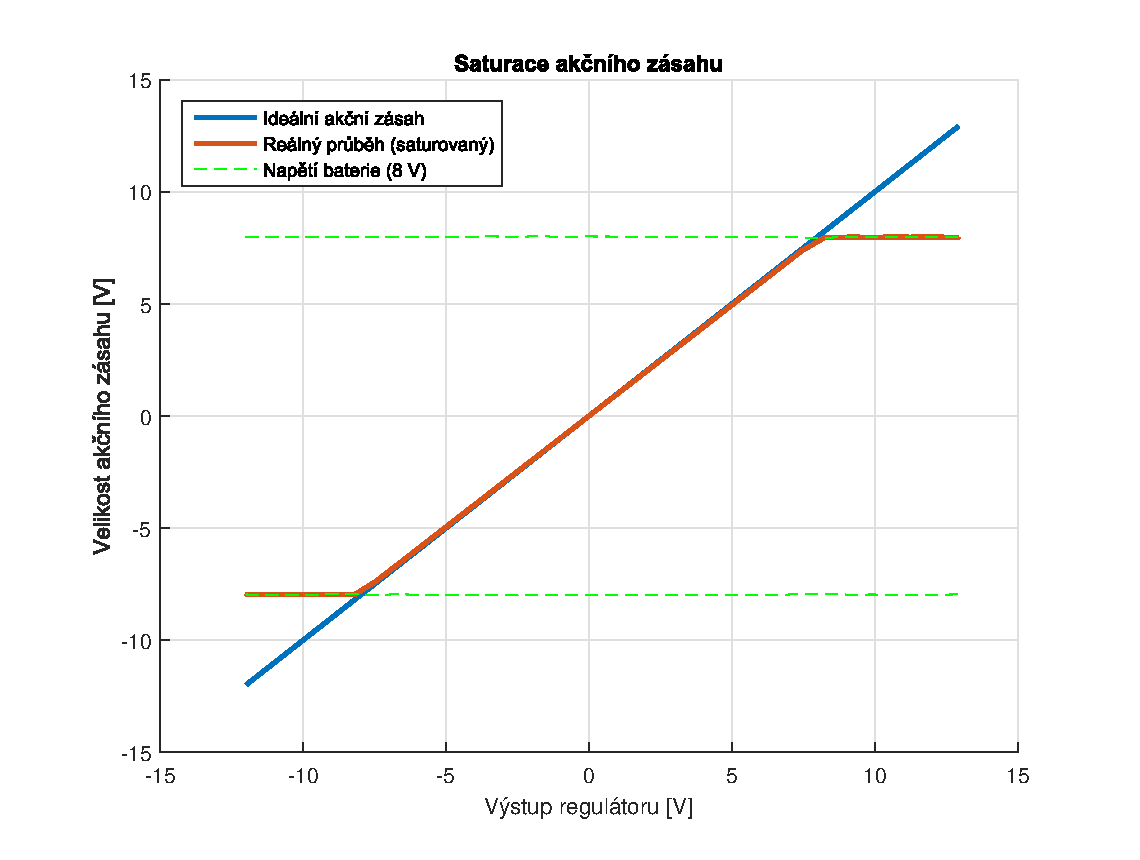
\includegraphics[width=\linewidth]{pwm_saturace.eps}}
    \caption{Saturace akčního zásahu vlivem konečného napětí baterie}
    \label{fig:pwm_saturace}        
\end{figure}

Na obrázku \ref{fig:pwm_saturace} je patrná první statická nelinearita -- při plné střídě PWM lze na motory přiložit nejvýše $\pm U_{bat}$,
kde $U_{bat}$ je okamžité napětí baterie. Velikost akčního zásahu je tak omezena na interval $u \in [-U_{bat}, U_{bat}]$.
S ohledem na změřené parametry $U_\text{max}$, $I_\text{max}$ a $R_\text{in}$ napájecího zdroje zanesené v tabulce \ref{tab:konstanty} lze určit,
že maximální úbytek napětí na vnitřním odporu baterie bude $U_{drop} = R_\text{in} \cdot I_\text{max} = 195~\si{\milli\volt}$.
Protože se bude segway provozovat vždy jen krátce po plném nabití, lze bez velké chyby pesimisticky odhadnout $U_{bat} = 8$ \si{V}.
Ve standardních podmínkách bude činnost segwaye ukončena dříve, než výstupní napětí baterie stihne poklesnout na napěťovou hladinu 8 \si{V}.

\begin{figure}[htbp]
    \centerline{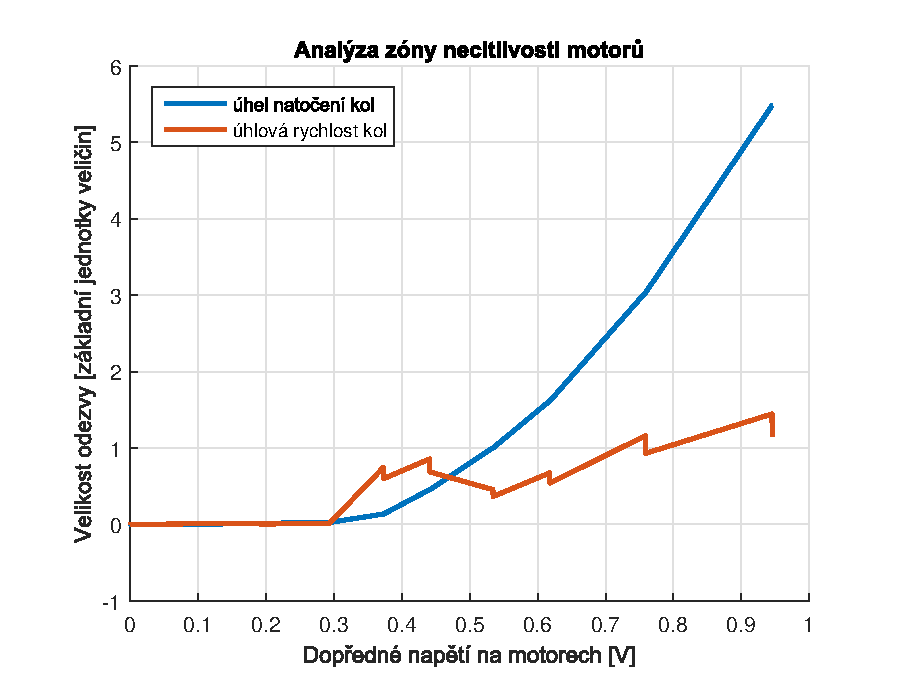
\includegraphics[width=\linewidth]{deadzone_motory_vpred.eps}}
    \caption{Měření reakce soustavy na malé kladné hodnoty akčního zásahu}
    \label{fig:deadzone_vpred}        
\end{figure}

\subsection{Pásmo necitlivosti}
Na motorech lze identifikovat pásmo necitlivosti při aplikaci napětí blízkého nule. Při velmi nízké hodnotě
akčního zásahu není schopen kroutivý moment motorů překonat statické tření v motoru.
Šířku pásma necitlivosti lze určit připojením napěťové rampy a sledováním závislosti úhlové rychlosti kol na napětí.
Opakováním pro rampu s kladnou a zápornou derivací lze určit šířku pásma necitlivosti na obě strany od nuly.

Odezva na rostoucí rampu napětí je vykreslena v grafu \ref{fig:deadzone_vpred}. Odečtením lze určit,
že pásmo necitlivosti je široké 0.3 \si{V} ve směru kladných napětí odpovídajících jízdě robota dopředu. 

\begin{figure}[htbp]
    \centerline{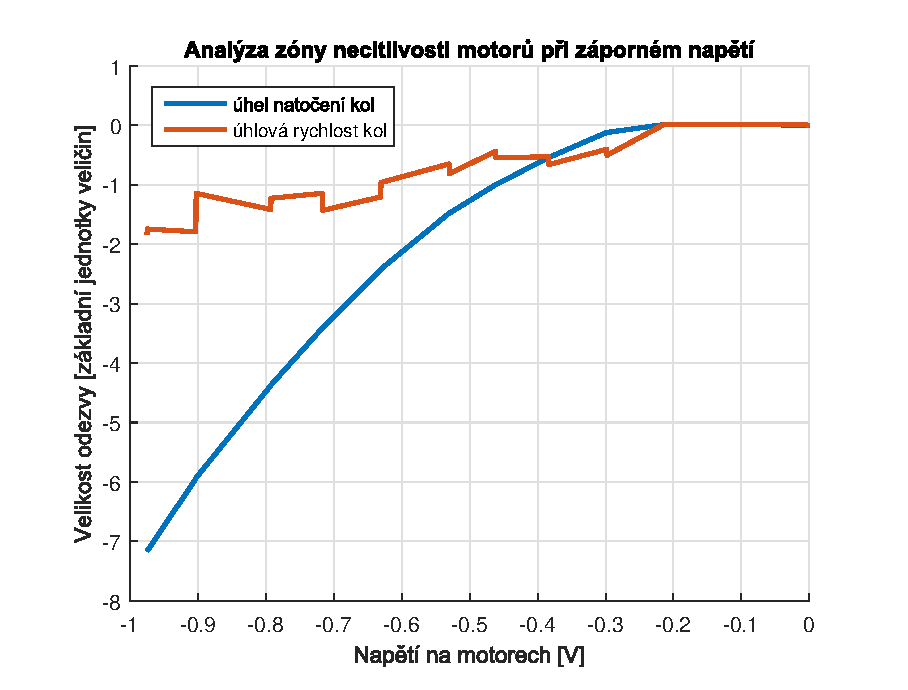
\includegraphics[width=\linewidth]{deadzone_motory_vzad.eps}}
    \caption{Měření reakce soustavy na malé záporné hodnoty akčního zásahu}
    \label{fig:deadzone_vzad}        
\end{figure}

Jízdě dozadu odpovídá pásmo necitlivosti vykreslené na grafu \ref{fig:deadzone_vzad}, ze kterého
lze odečíst šířka pásma necitlivosti přibližně 0.22 \si{V}. Motory jsou tedy necitlivé
na akční zásah
\begin{equation}
    u_{deadzone} \in [-0.22, 0.3] ~\si{V}.
    \label{eq:deadzone}
\end{equation}

\subsection{Saturace stavů systému}

Ze stavových proměnných soustavy může být saturováno $x_2$ odpovídající úhlu náklonu od svislice $\psi$.
Hodnoty $\psi = \pm \frac{\pi}{2}$ odpovídají stavu, kdy robot spadne a položí se na plocho na konstrukci těla.
Jedná se o stabilní ekvilibria, z hlediska řešení úlohy jsou ale silně nežádoucí. Pakliže je cílem udržet segway ve svislé poloze,
musí se soustava těmto dvěma stavům vyhnout za každou cenu. Proto není tato saturace pro návrh řízení nijak podstatná.

Proměnná $x_1$ odpovídající úhlu koleček $\theta$, ani stavy $x_{3,4}$ odpovídající úhlovým rychlostem $\dot{\theta}$ a $\dot{\psi}$,
nemohou být saturovány. Úhlová dráha uražená kolečky je obecně neomezená, stejnětak obě úhlové rychlosti.

Saturovatelná je rovněž vzdálenost od překážky $d$. Ultrazvukový senzor vzdálenosti má rozlišení 8 bitů s krokem 1 \si{\centi\metre},
hodnota $d$ tak bude v každý okamžik saturována na interval $d \in \left[0, 255\right]$. Tato saturace však není pro návrh řízení podstatná --
pakliže je totiž překážka více jak $2.5 \text{\si{\metre}}$ daleko, nezáleží již příliš na přesné vzdálenosti.

\subsection{Dynamika motorů}

Pro identifikaci parametrů motorů byl na vstup motorů přiložen skok napětí z $0$ na $60$ \% střídy PWM.
Při uvážení $U_{bat}$ dle sekce \ref{sec:ubat} to odpovídá vstupnímu napětí $U_\text{in} = \frac{60}{100} U_{bar} = 4.8$ \si{\volt}.
Změřená odezva je vykreslena na obrázku \ref{fig:motor_skok}. V průběhu měření vypadla část vzorků mezi časy $250~\text{\si{\milli\second}}$ 
a $380~\text{\si{\milli\second}}$. Pro identifikaci je tak potřeba uvážit jen validní část průběhu.

\begin{figure}[htbp]
    \centerline{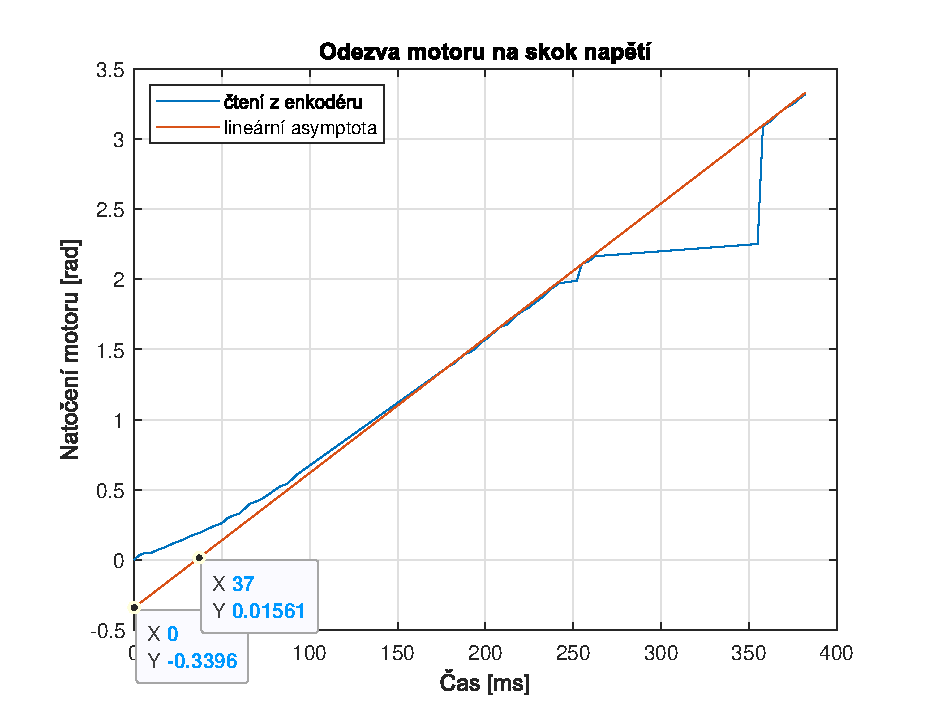
\includegraphics[width=\linewidth]{motor_skok.eps}}
    \caption{Odezva motoru na skok}
    \label{fig:motor_skok}        
\end{figure}

Tvar odezvy poukazuje na soustavu druhého řádu typu jedna bez nul, jejíž přenos má tvar
\begin{equation}
    G(s) = \frac{k}{s(Ts+1)},
    \label{eq:servo_prenos}
\end{equation}
kterému v časové oblasti přísluší průběh odezvy na skok
\begin{equation}
    h(t) = \underbrace{k(t-T)}_{\text{asymptota pro t $\to \infty$}} + \underbrace{Tk e^{\frac{-t}{T}}}_{\text{přechodový děj}},
    \label{eq:servo_odezva}
\end{equation}
kde směrnici asymptoty $k$, a časovou konstantu $T$ lze dále konkretizovat metodou \textit{grey box}.
Směrnice asymptoty
\begin{equation}
    k_{60\%} = \frac{\Delta y}{\Delta x} = \frac{0.35521}{0.037} = 9.6~\text{\si{\radian\per\second}}
\end{equation}
odpovídá úhlové rychlosti otáčení motoru při použité střídě $60$ \%. Při plné střídě spínání nezatížených motorů lze dosáhnout rychlosti
\begin{equation*}
    \omega_\text{max} = k_{60\%} \cdot \frac{100}{60} = 16~\text{\si{\radian\per\second}} \approx 152~\text{RPM},
\end{equation*}
což souhlasí s výsledky prezentovanými ve Figure 6-3 v \cite{model_based_design}.
V čase $T$ musí mít asymptota nulovou hodnotu -- odečtením z grafu je vidět $T = 0.037$ \si{\second}.
Protože testovací vstupní signál neměl jednotkovou amplitudu, je potřeba nalezené parametry ještě přeškálovat vydělením $U_\text{in}$. 
Identifikované přenosy servo motoru z řídicího napětí $u$ na úhel natočení $\theta$ a úhlovou rychlost $\dot{\theta}$ koleček mají tvar
\begin{equation}
    \begin{aligned}
        G_{u\to\theta}(s) &= \frac{1}{U_\text{in}} \frac{9.6}{s(0.037s + 1)}   &=  \frac{54.0541}{s(s+27.0270)}, \\
        G_{u\to\dot{\theta}}(s) &= sG_{u\to\theta}(s) &= \frac{54.0541}{s+27.0270}.
    \end{aligned}
\end{equation} 

Dynamika motorů je stabilní a ve srovnání s dynamikou zbytku soustavy diktovanou póly vypsanými v rovnici \eqref{eq:unstable_poles} zanedbatelná.
Integrační charakter pólu v počátku i poloha kolem bodu $-6$ je několikrát pomalejší než pól v bodě $-27$ a dynamika motorů tak nebude zásadně ovlivňovat soustavu.

\section{Porovnání modelu a systému}

Rovnice \eqref{eq:pohyb1_easy} až \eqref{eq:motor2_easy} byly implementovány jako simulinkový model vyobrazený na schématu \ref{fig:simulink_nelin_model}.
V nelineárním modelu je zohledněna saturace náklonu $\psi$ na interval $[-\frac{\pi}{2}, \frac{\pi}{2}]$ rad, stejnětak i pásmo necitlivosti motorů $u_{deadzone}$.
Paralelně byl zařazen blok \textit{State space} obsahující linearizovaný model představovaný maticemi dle rovnice \eqref{eq:matice_linearizovane}.
\subsection{Odezva na skok}
Při první simulaci byl nelineární i linearizovaný model
vystaven jednotkovému skoku vstupního napětí $u$ v čase 1 \si{\second}. Průběhy stavových veličin jsou zobrazeny na obrázku \ref{fig:porovnani_skok}.
Pro přehlednost není zobrazen průběh stavu $x_1$ (úhel koleček $\theta$), neboť jeho hodnota není pro úlohu balancování důležitá.
\begin{figure}[htbp]
    \centerline{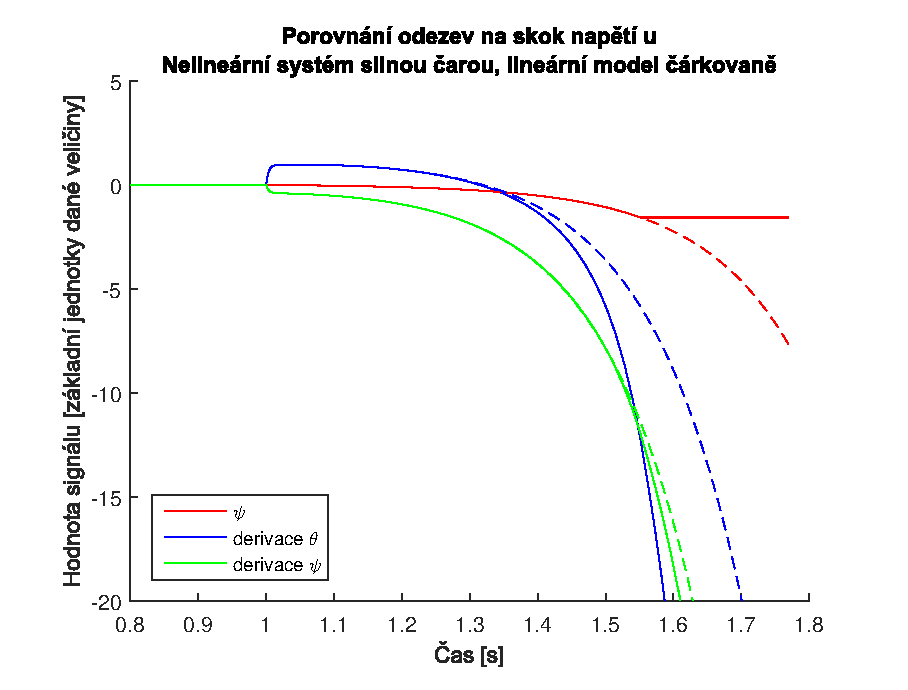
\includegraphics[width=\linewidth]{porovnani_skok.eps}}
    \caption{Simulace odezvy na skok napětí}
    \label{fig:porovnani_skok}        
\end{figure}
Oba modely mají stejný charakter časových průběhů, jsou velmi nestabilní a rychle divergují.
V čase cca. $1.6~\si{\second}$ nastane modelově pád robota na zem a hodnota $\psi$ je dále neměnná -- reálný nelineární systém by setrvával ve stabilním ekvilibriu.
Pakliže zůstanou dodrženy podmínky linearizace na blízkost pracovnímu bodu, odpovídá linearizovaný model modelu nelineárnímu.

\subsection{Odezva na rampu}
V případě připojení rampy na vstup $u$ soustavy se projeví pásmo necitlivosti na motorech. Na obrázku \ref{fig:porovnani_rampa} jsou pro porovnání
vykresleny odezvy na rampu vstupního signálu s předpisem $u(t) = t$ (sklon 1). 
\begin{figure}[htbp]
    \centerline{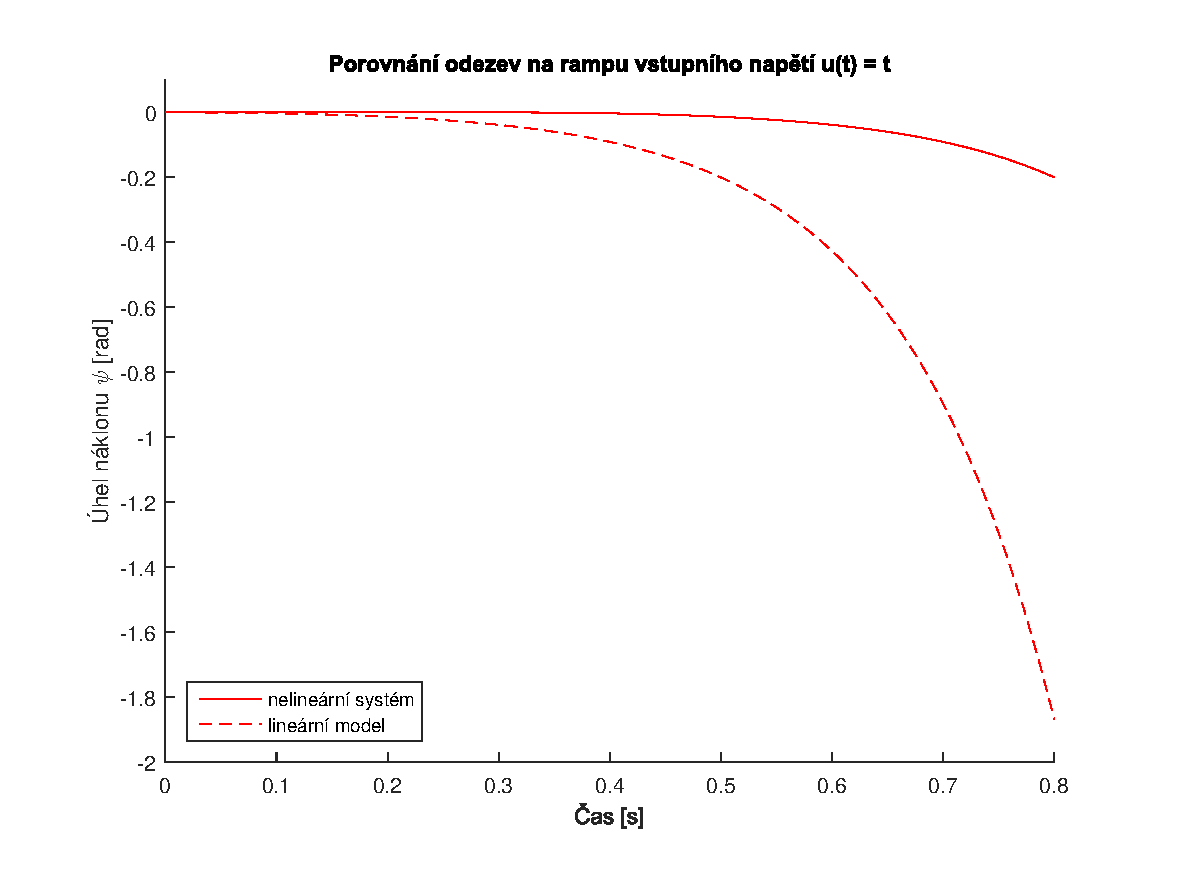
\includegraphics[width=\linewidth]{porovnani_rampa.eps}}
    \caption{Simulace odezvy na rampu napětí}
    \label{fig:porovnani_rampa}        
\end{figure}
Lineární model nerespektuje psámo necitlivosti popsané v rovnici \eqref{eq:deadzone}, pročež se jeho stav začne měnit bezprostředně po startu,
zatímco nelineární systém je v klidu až do okamžiku, kdy napětí $u$ překoná hranici pásma necitlivosti.

\section{Návrh řízení}
Matice soustavy $\textbf{A}$ má vlastní čísla 
\begin{equation}
	\text{eig}(\mathbf{A}) =
	\begin{cases}
        0 \\
        -6.4178 \\
        7.2604 \\
        -231.6811
    \end{cases},
    \label{eq:unstable_poles}
\end{equation}
jeden mód je na mezi stability a jeden je silně nestabilní. Za účelem splnění požadavků na chování bude potřeba před soustavu zařadit regulátor $K(s)$ generující
akční zásah $u$ a uzavřít stabilizující zpětnovazební smyčku.
\subsection{Kompenzace nelinearit}
 Pro částečnou kompenzaci pásma necitlivosti motorů dle \eqref{eq:deadzone} je mezi výstup regulátoru a vstup soustavy
zařazen blok \textit{Coulombic and viscous friction} s parametry $\text{Offset} = 0.15$, $\text{Gain} = 1$. Velikost offsetu byla laděna
experimentálně s cílem zajistit plynulé průběhy akčního zásahu. Na obrázku \ref{fig:bez_kompenzace_treni} jsou vidět body, v nichž nejsou průběhy stavů hladké.
\begin{figure}[htbp]
    \centerline{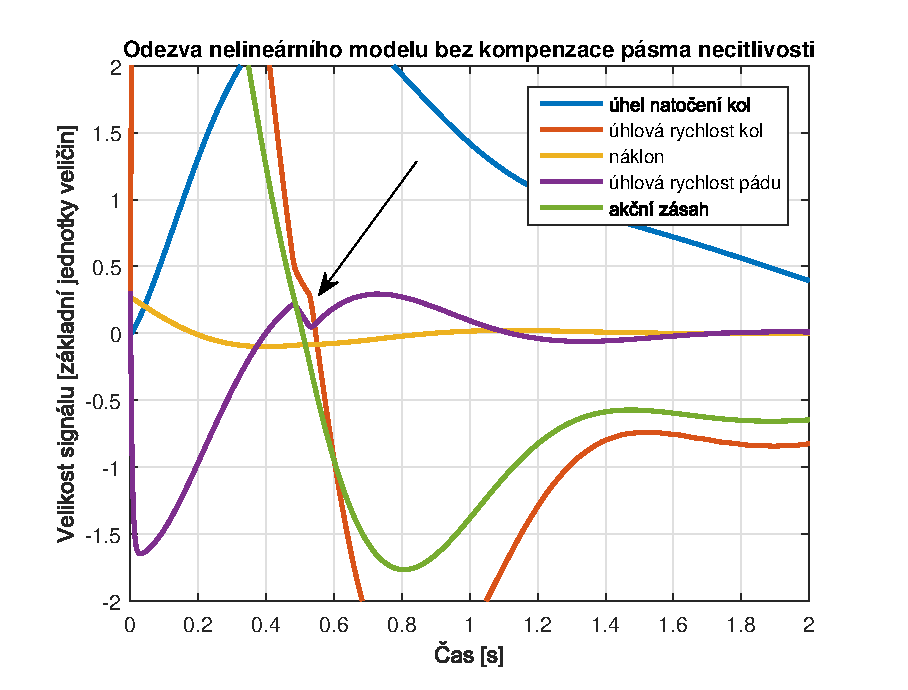
\includegraphics[width=\linewidth]{regulace_bez_kompenzace_treni.eps}}
    \caption{Neexistence derivace stavových proměnných v některých bodech kvůli nekompenzovanému statickému tření}
    \label{fig:bez_kompenzace_treni}        
\end{figure}

Bez kompenzace pásma necitlivosti měl segway tendenci k oscilacím kolem pracovního bodu, neboť akční zásah $u$ byl schopen pohnout motory
až od jisté velikosti, kdy stavy segwaye byly již daleko vychýleny od nulové polohy.
Offset vyšší jak $0.4$ rovněž způsoboval oscilace, neboť stačila malá regulační odchylka stavových proměnných k vygenerování velkého akčního zásahu,
jenž přestřelil stabilní polohu.
Z vytyčeného intervalu přípustných offsetů byla iteračně aproximační metodou vybrána hodnota $0.15$,
neboť experimentálně zajišťovala nejplynulejší pohyb segwaye.
Zásadním problémem pro přesnější kompenzaci pásma necitlivosti je jeho asymetrie patrná z \eqref{eq:deadzone}. Pro dosažení lepších výsledků by bylo možné
použít různý offset v závislosti na hodnotě $\text{sign}(u)$, jednalo by se však o zbytečné zesložitění přinášející jen malé vylepšení
ve srovnání s výše popsanou symetrickou kompenzací.
S použitím kompenzace o výše uvedených parametrech byly průběhy signálů vyhlazeny, jak je patrno na obrázku \ref{fig:kompenzace_treni}. 


\begin{figure}[htbp]
    \centerline{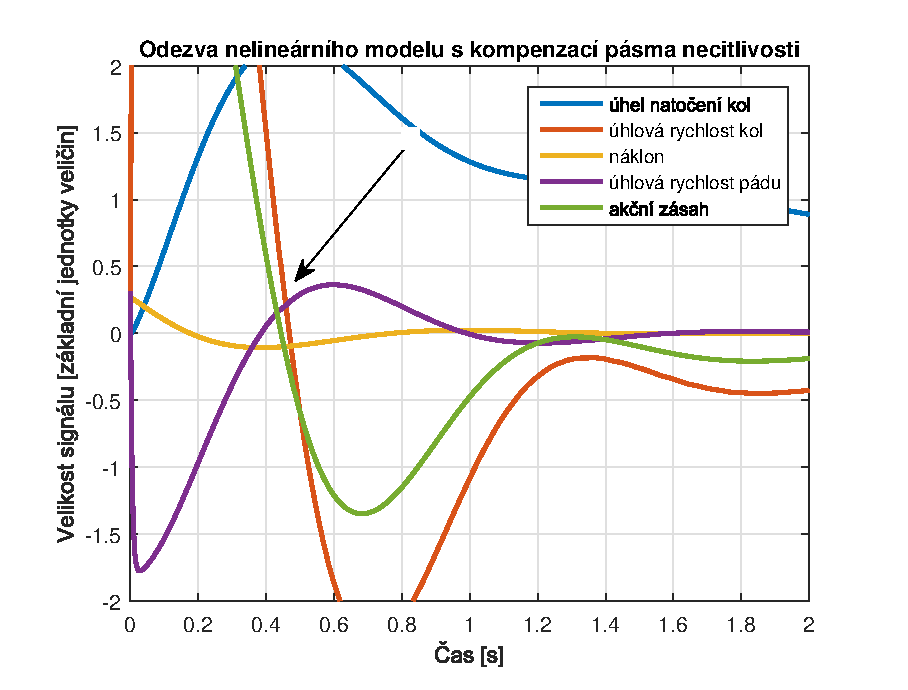
\includegraphics[width=\linewidth]{regulace_kompenzace_treni.eps}}
    \caption{Vyhlazené průběhy stavových proměnných díky kompenzaci tření}
    \label{fig:kompenzace_treni}        
\end{figure}

\subsection{Základní balancování stavovou zpětnou vazbou}
Pro úlohu stabilizace robotu v nestabilní svislé poloze postačuje použití stavové zpětné vazby s regulátorem $K~=~\left[ k_1 ~ k_2 ~ k_3 ~ k_4 \right]$
pro $k_i \in \mathbb{R}$, jehož zapojení do schématu je na obrázku \ref{fig:stavova_zv} zapůjčeném z \cite{img:full_state_feedback}.
Pro tuto topologii systému je akční zásah lineární kombinací stavových proměnných soustavy, neboť
\begin{equation}
    u = K \cdot \vec{x} = \sum_{i=1}^4 k_i x_i.
\end{equation}

\begin{figure}[htbp]
    \centerline{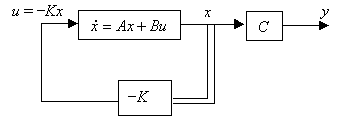
\includegraphics[width=\linewidth]{full_state_feedback_schematic.png}}
    \caption{Blokové schéma zapojení stavové zpětné vazby}
    \label{fig:stavova_zv}        
\end{figure}

Stavová zpětná vazba je pouze proporcionální a nevnáší do soustavy další dynamiku. Protože platí
\begin{equation}
    \text{rank}(\text{ctrb}(\mathbf{A}, \mathbf{B})) = 4,
\end{equation}
je soustava plně řiditelná a stavová zpětná vazba umístí všechny čtyři póly $p_i$ pro $i \in \left\{1, 2,3,4\right\}$ uzavřené smyčky.

V zadání úlohy jsou stanoveny cíle na dynamiku -- rychlý čas ustálení $T_s$ (například $T_s = 1.5$ \si{\second}) a maximální překmit $OS = 20$ \%.
Tyto požadavky  splňuje komplexně sdružená dvojice pólů $p_{1,2} = -0.0267 \pm 0.0521i$.
Třetí pól je ponechán na svém místě v bodě $p_3 = -231$. Čtvrtý pól $p_4$ je za účelem stabilizace záhodno umístit blízko počátku.
Byly nalezeny dvě významné polohy:
\begin{enumerate}
    \item \textbf{Čistý integrátor} $p_4 = 0$ v přenosu uzavřené smyčky vedl na eliminaci stavu $x_1$ ze stavové zpětné vazby.
    Nezávislost výstupu regulátoru 
    \begin{equation*}
        K_1 = \begin{bmatrix}
            0 & -11.1715  & -0.8910  & -2.1115
        \end{bmatrix}
    \end{equation*}
    na $\theta$ zajistila translační invarianci stability. Segway tedy bylo možno dotlačit do nové polohy, v níž se opět stabilizoval. Nezávislost na $\theta$
    však byla souběžně i nevýhodou, neboť robot vlivem malých leč nenulových regulačních odchylek během času pomalu couval, až narazil na překážku v místnosti.
    Výsledky simulace tohoto chování jsou vyneseny na obrázku \ref{fig:stavova_K2_nelin}.

    \item \textbf{Pomalý mód} $p_4 = -0.5$ projevil nejlepší vlastnosti co se týče řízení stavových veličin k nule. Odpovídající regulátor
    \begin{equation*}
        K_2 = \begin{bmatrix}
            -0.1883 & -12.4845 &  -0.9211 &  -2.1853
        \end{bmatrix}
    \end{equation*}
    zohledňuje i úhel natočení kol $\theta$ a tudíž udržuje robota ve stabilní poloze na jednom místě.
\end{enumerate}

\begin{figure*}[h!]
    \centering % <-- added
    \begin{subfigure}{0.45\textwidth} 
        \centerline{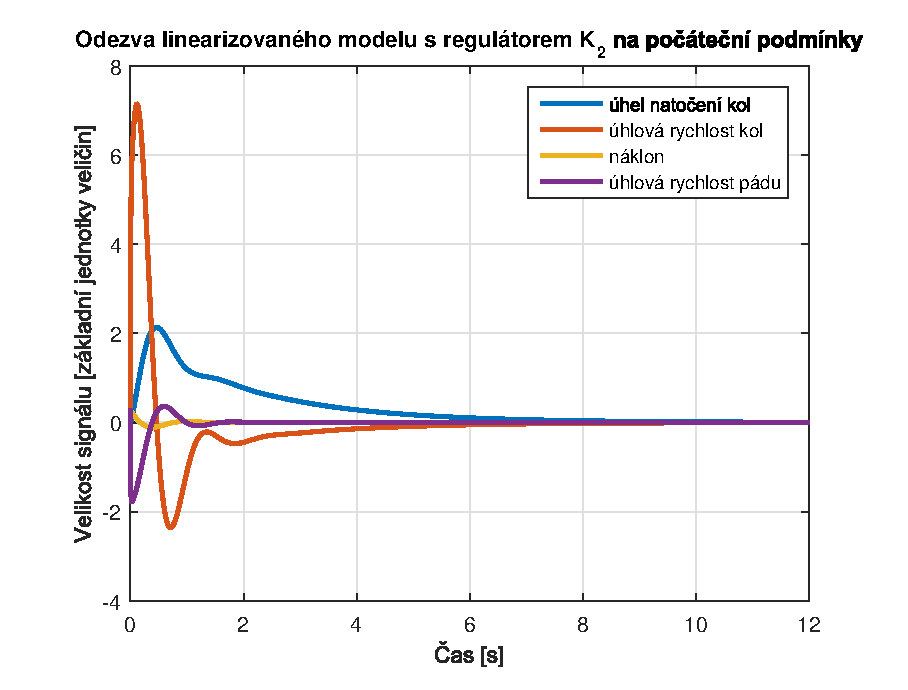
\includegraphics[width=\linewidth]{stavova_K2_lin.eps}}
        \caption{Linearizovaný model a $K_2$ \\ dokonalé uklidnění systému}
        \label{fig:stavova_K2_lin}        
    \end{subfigure}\hfil
    \centering % <-- added
    \begin{subfigure}{0.45\textwidth}
        \centerline{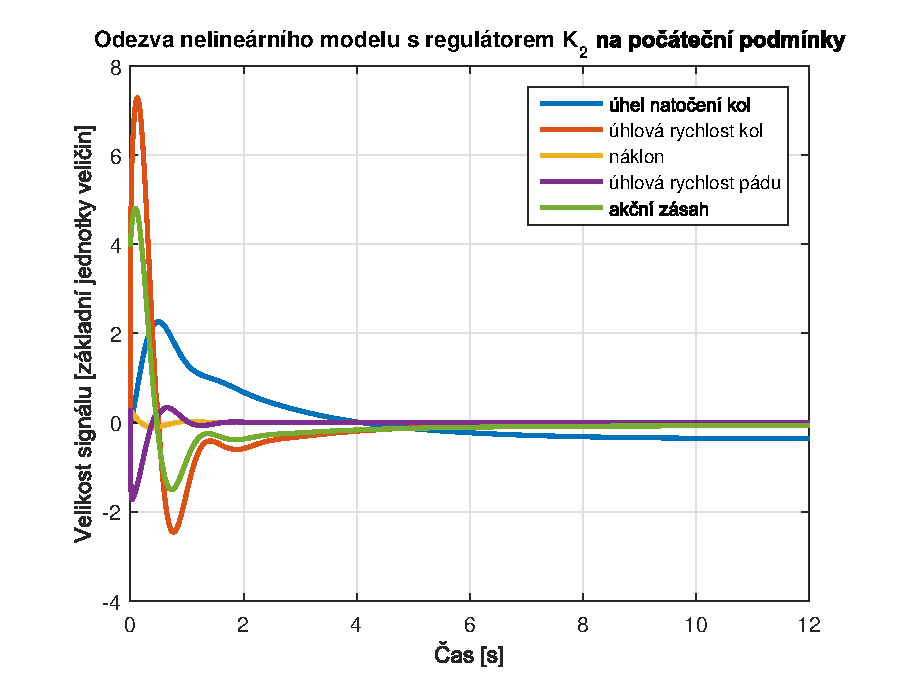
\includegraphics[width=\linewidth]{stavova_K2_nelin.eps}}
        \caption{Nelineární systém a $K_2$ \\ malá neměnná chyba, segway necestuje}
        \label{fig:stavova_K2_nelin}        
    \end{subfigure}\hfil
    
    
    \medskip
    
    \centering % <-- added
    \begin{subfigure}{0.45\textwidth} 
        \centerline{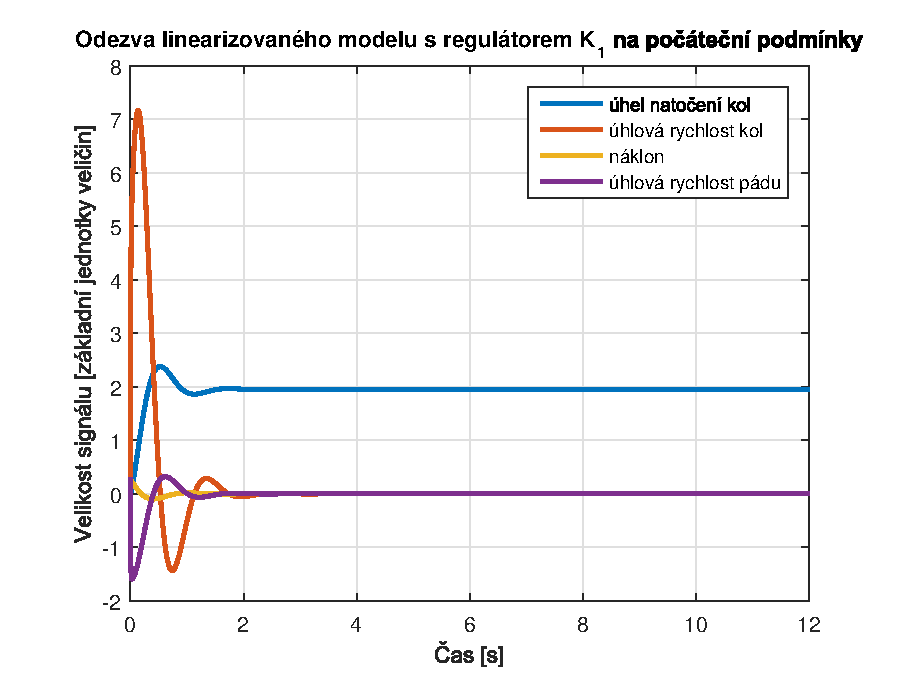
\includegraphics[width=\linewidth]{stavova_K1_lin.eps}}
        \caption{Linearizovaný model a $K_1$ \\ velká neměnná chyba v ustáleném stavu}
        \label{fig:stavova_K1_lin}        
    \end{subfigure}\hfil
    \centering % <-- added
\begin{subfigure}{0.45\textwidth}
    \centerline{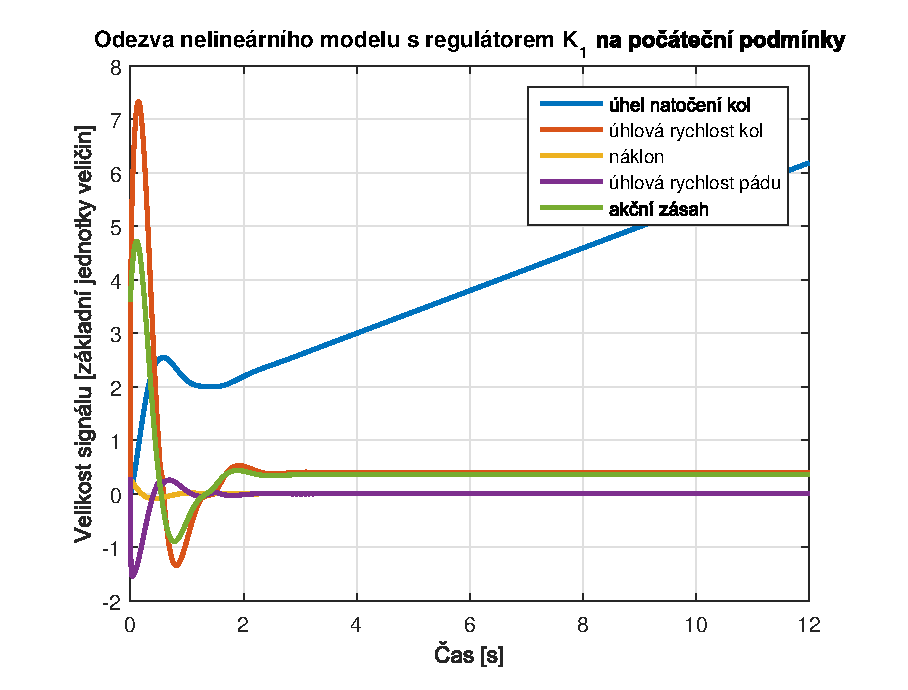
\includegraphics[width=\linewidth]{stavova_K1_nelin.eps}}
    \caption{Nelineární systém a $K_1$ \\ segway postupně odjíždí ($\theta$ diverguje)}
    \label{fig:stavova_K1_nelin}        
\end{subfigure}\hfil

\caption{Srovnání stavových regulátorů $K_{1,2}$ pro ustálení z nenulových počátečních podmínek}
\label{fig:charakteristiky}
\end{figure*}

Oba stavové regulátory zajistí teoreticky stabilní uzavřenou zpětnovazební smyčku, z definice by tedy měly všechny možné počáteční
podmínky pro stavové proměnné odeznít s rostoucím časem do nuly. Pro experiment byly zvoleny počáteční podmínky
\begin{equation*}
    \begin{bmatrix}
        \theta_0 & \psi_0 & \dot{\theta}_0 & \dot{\psi}_0
    \end{bmatrix} = \begin{bmatrix}
        0 & 15~\si{\degree} & 0 & 18~\si{\degree\per\second}
    \end{bmatrix}
\end{equation*}
odpovídající vnější poruše, kdy například vlivem srážky s překážkou segway zastaví $\dot{\theta} = 0$ a začne přepadávat $\dot{\psi} \neq 0$.


Na obrázcích \ref{fig:stavova_K2_lin} a \ref{fig:stavova_K2_nelin}
jsou k porovnání časové průběhy odezev linearizovaného modelu s regulátorem $K_2$ i nelineárního modelu se zapojeným regulátorem $K_2$ na nenulové počáteční podmínky.
Přechodové děje na počátku nejsou příliš zajímavé, důležitý je ustálený stav. Zatímco linearizovaný model skutečně s použitím regulátoru $K_2$ všemi svými stavy 
odezní do nuly, simulace nelineárního modelu ukazuje na jistotou nenulovou konstantní hodnotu úhlu natočení koleček $\theta$. Tento nedostatek však není nijak omezující
a je snadno akceptovatelný. 


Průběhy ze simulace použití stavového regulátoru $K_1$, jehož nasazení umístí jeden pól uzavřené smyčky do počátku $s$ roviny, jsou vykresleny na obrázkách 
\ref{fig:stavova_K1_lin} a \ref{fig:stavova_K1_nelin}. Charaktery průběhů jsou shodné s ději pro regulátor $K_2$, liší se ovšem ustálený stav -- integrátor v přenosu
soustavy způsobí konstantní nenulovou hodnotu v případě linearizovaného modelu a v případě nelineárního modelu dokonce úhel natočení koleček pomalu diverguje.

Stavovou zpětnou vazbou se podařilo dosáhnout rozumné stability odezvy na počáteční podmínky. Protože je SZV inherentně proporcionální, nelze očekávat
dokonalé vlastnosti odezvy na poruchy v soustavě. Základní je garantovat stabilitu, je očekávatelná nenulová ustálená regulační odchylka,
neboť proporcionální regulace není schopná zajistit asymptotické sledování. Na obrázku \ref{fig:porucha_stavova_ZV} je vykreslen průběh simulovaných signálů ve smyčce nelineárního
systému a stavového regulátoru $K_2$, kde v čase $t = 20~\text{\si{\second}}$ nastane jednotkový skok poruchy.
Segway se podle nastavené $T_s$ vrátí zpět do svislé polohy, ovšem vlivem působící poruchy dojde ke stabilizaci soustavy v jiném bodě stavového postoru ($\theta \neq 0$).
Regulátor musí aktivně generovat akční zásah pro kompenzování poruchy tak, aby na vstupu soustavy byly hodnoty blízké nule.


\begin{figure}[h!]
    \centerline{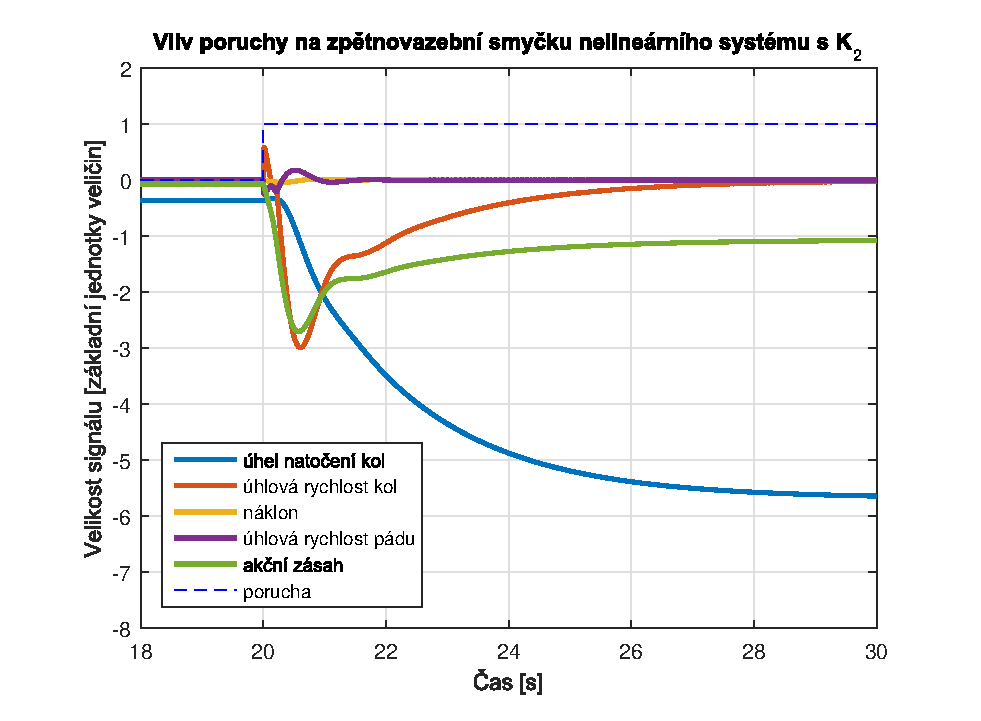
\includegraphics[width=\linewidth]{stavova_ZV_porucha.eps}}
    \caption{Neschopnost proporcionální stavové zpětné vazby asymptoticky sledovat poruchu}
    \label{fig:porucha_stavova_ZV}        
\end{figure}

\subsection{Optimalizace stabilizující stavové zpětné vazby}

Lepší vlastnosti odezvy na poruchu by mohlo zajistit integrální řízení, jehož zavedení by však navýšilo řád soustavy a způsobilo tak nežádoucí zesložitění.
Při experimentálních testech stability fyzickým vyváděním segwaye ze stabilní polohy konal problémy velký překmit ustalování, pakliže bylo vyvoláno
několik poruch rychle po sobě. Segway se nechal rozkmitat a stal se nestabilním. Pro své obecně lepší vlastnosti byl regulátor $K_1$ zvolen jako základ
pro další zlepšování. Cíl stabilizovat systém i v přítomnosti mnoha rychlých poruch vyžaduje upravení požadavků na dynamiku -- experimentálně byly zvoleny
požadavky $T_s = 1~\text{\si{\second}}$ a $OS = 8~\%$ na póly $p_{1,2}$. Póly $p_{3,4}$ jsou ponechány v týchž polohách jako pro regulátor $K_1$.
Výsledný regulátor
\begin{equation*}
    K_3 = \begin{bmatrix}
        -0.2243 & -17.1901 &  -1.0080 &  -2.4071
    \end{bmatrix}
\end{equation*}
zajistil jen zanedbatelné popojíždění segwaye srovnatelné s regulátorem $K_1$ při dosažení velice dobré stability a schopnosti se vypořádat i s dynamickými změnami rozložení
hmotnosti například pověšením zátěže na jednu stranu robota. Z experimentů s tímto regulátorem byla pořízena videodokumentace přiložená k této zprávě.
Další snižování parametru $T_s$ není příliš možné s ohledem na velikost akčního zásahu patrnou např. na obrázku \ref{fig:stavova_K2_nelin}, na němž je vidět že již pro
konzervativnější volbu $T_s = 1.5~\text{\si{\second}}$ je potřebný akční zásah větší než polovina maximální hodnoty omezené saturací.   
Volba ještě menšího $T_s$ obecně vyžaduje agresivnější a rychlejší regulátor, který všek v našem kontextu velmi rychle narazí na saturaci akčního zásahu do soustavy.


\subsection{Sledování vzdálenosti od překážky}

První pokus o řízení pomocí vzdálenosti od překážky $d$ byl návrh proporcionálního regulátoru pro svou jednoduchou integrovatelnost do systému.
Použitá stavová zpětná vazba spolehlivě udržuje robota ve stavovém prostoru poblíž bodu $\vec{o}$. Pomocí vztahu \eqref{eq:vzdalenost} se nabízí přímočarý
způsob řízení veličiny $d$ -- dopočíst hodnotu $\theta$, pro kterou bude splněno $d = d_{ref}$, a následně robota dovést na tento nový úhel koleček. 


Na obrázku \ref{fig:vzdalenost_P} je vykreslen časový průběh $d(t)$ z minutového spuštění robota.
\begin{figure}[htbp]
    \centerline{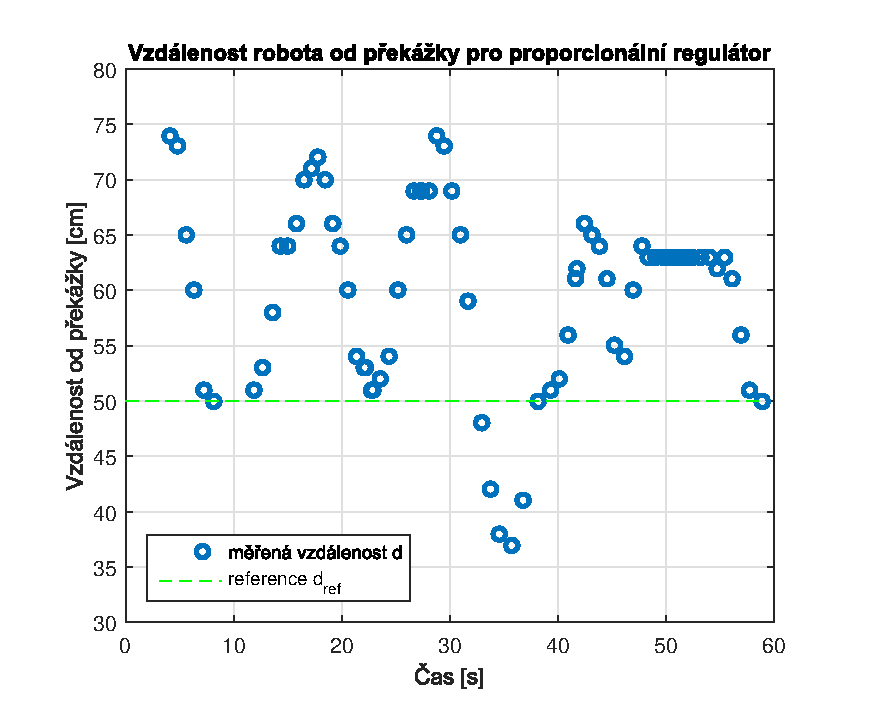
\includegraphics[width=\linewidth]{vzdalenost_od_prekazky_proporcionalni.eps}}
    \caption{}
    \label{fig:vzdalenost_P}        
\end{figure}
Proporcionální regulátor nedokázal zajistit ustálenou regulační odchylku. Při poruše (představované šťouchnutím do robota)
se proporcionální regulace nedokázala vrátit na nastavenou referenční hodnotu $d_\text{ref} = 50~\text{\si{\centi\metre}}$.
Pro zajištění nulové regulační odchylky bude nezbytná integrační složka.


Výše diskutované nevýhody P regulátoru řeší regulátor typu PI.  

\section{Závěr}
V rámci práce se podařilo úspěšně ověřit validitu matematického modelu LEGO segwaye jako inverzního kyvadla.
Nalezený linearizovaný model dostatečně aproximuje dynamiku skutečného nelineárního systému v okolí pracovního bodu ve svislé pozici,
takže jej lze plně využít pro návrh řízení. Důkladné rozebrání několika možností regulace stavovou zpětnou vazbou umožňuje
hlubší vhled do problematiky stabilizace nelineárního systému včetně kompenzování neideálních vlastností.
Protože je v případě modelování kinematiky dvoukolového vozítka pojem stavů velmi intuitivní, je modelování systému stavovým popisem
hodno doporučení i pro navazující práce.  Stěžejním závěrem je samotné zdařilé splnění zadané úlohy.
Lze konstatovat, že mnoho stupňů volnosti stavové zpětné vazby je dostačujících pro plnění rozmanitých požadavků na dynamiku řízeného procesu
lišících se v oblasti časové (parametry jako $T_s$, $OS$) i konkrétních polohách pólů.

Využité metody návrhu regulátorů byly spíše základní, v navazující práci by bylo vhodné rigorozně odvodit -- nebo alespoň
přesně vyšetřit -- kritéria návrhu regulátorů zohledňující saturaci akčního zásahu.
K vyzkoušení stojí rovněž regulace \textit{deadbeat}, jež byla pro využití v této práci zavržena kvůli celkově rychlé dynamice a velké nestabilitě
systému v otevřené smyčce. Zpřesnění by si zasloužily rovněž konstantní parametry uvedené v tabulce \ref{tab:konstanty}.
Mnohé konstanty jako například $J_\varPhi$ či $L$ mají hodnoty stanoveny na základě předpokladu tuhého homogenního tělesa.
Opuštěním tohoto předpokladu by sice narostla složitost jejich přeného numerického vypočtení, ovšem z hlediska úlohy automatického řízení
by se jednalo o pouhou změnu konstant nijak neměnící složitost návrhu regulace.

V neposlední řadě by úloha stabilizace robota ve svislé poloze benefitovala z přesnějšího stanovení hranic pásem necitlivosti
motorů. Ve zprávě byla diskutována varianta symetrické a asymetrické kompenzace pásma necitlivosti, dále je ovšem potřeba zpochybnit
zamlčený předpoklad identického pásma necitlivosti na všech dostupných motorech. Hladký postoj robota by byl nezbytným předpokladem
pro nasazení například v úlohách stabilizace kamer nebo při přepravě křehkého zboží.



\begin{thebibliography}{9}
    
    \bibitem{model_based_design}
    Yorihisa Yamamoto, \emph{NXTway-GS Model-Based Design} 
    
    \bibitem{img:full_state_feedback} G. Goodwin, S. Graebe, M. Salgado, \emph{Control system design}, supplementary materials to book \url{http://www.csd.elo.utfsm.cl/simulations/pend_sim5.html}
    
\end{thebibliography}

\pagebreak
\section{Appendix}

Schémata a další přílohy z procesu návrhu řízení. Schémata jsou pouze orientační, kompletní simulinkové modely jsou přiloženy ke zprávě.

\begin{figure*}[htbp]
    \centerline{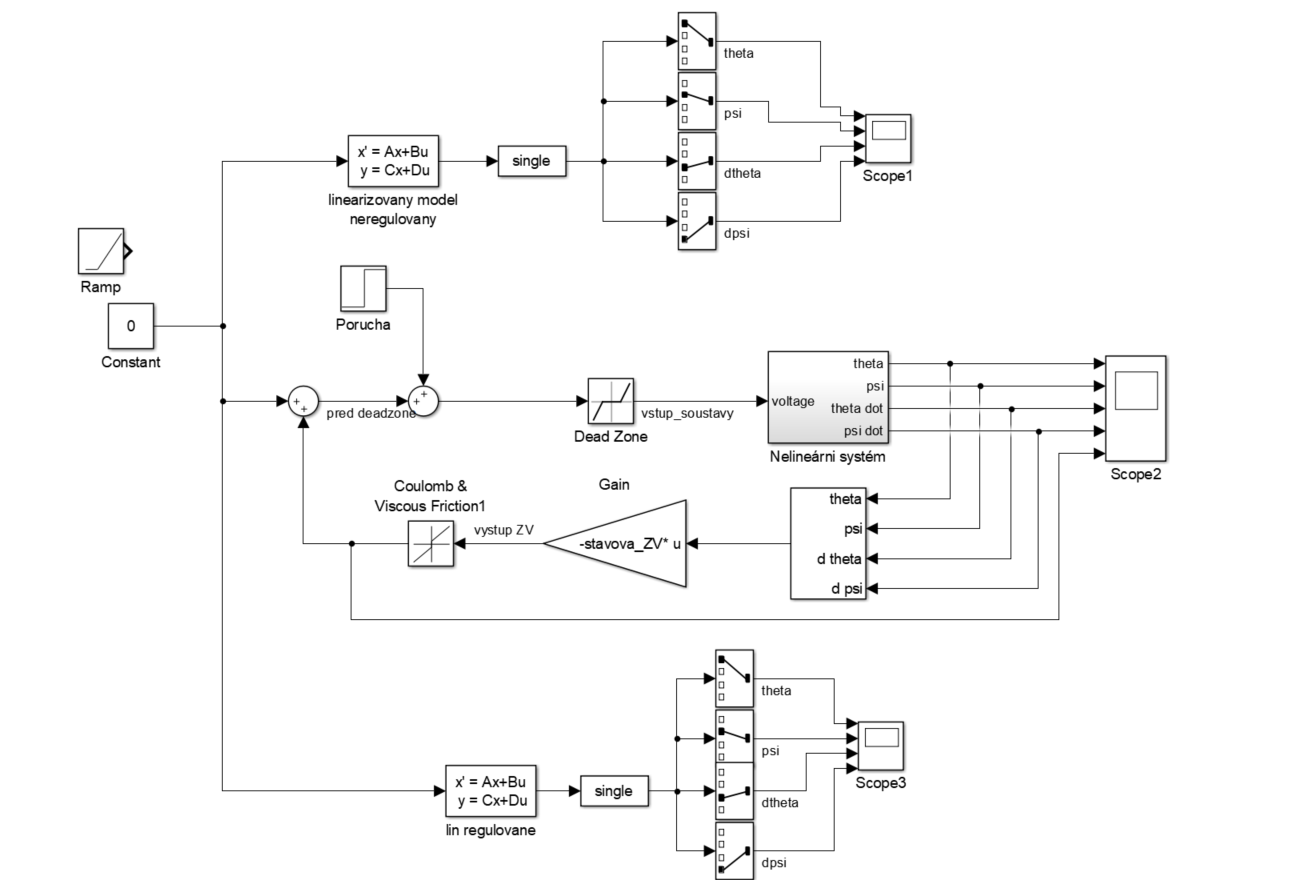
\includegraphics[width=\linewidth]{simulace_simulink.png}}
    \caption{Model programu SIMULINK používaný pro porovnání odezev a řízení linearizovaného a nelineárního modelu systému}
    \label{fig:simulink_simulace}        
\end{figure*}

\begin{figure*}[htbp]
    \centerline{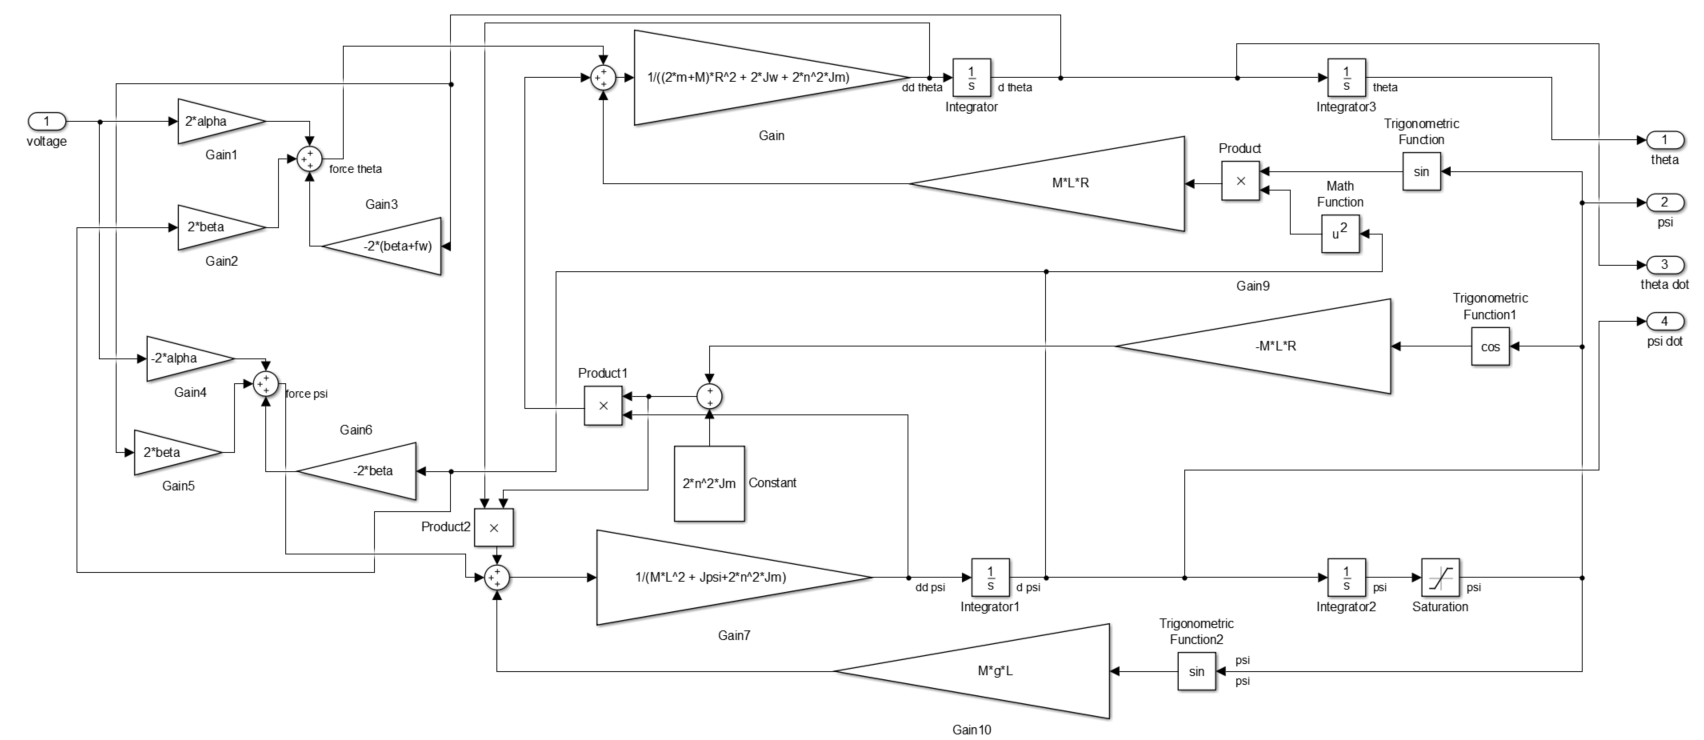
\includegraphics[width=\linewidth]{nelinearni_system_simulink.png}}
    \caption{Model programu SIMULINK implementující diferenciální rovnice \eqref{eq:pohyb1_easy} až \eqref{eq:motor2_easy}}
    \label{fig:simulink_nelin_model}        
\end{figure*}
\end{document}
